%  article.tex (Version 3.3, released 19 January 2008)
%  Article to demonstrate format for SPIE Proceedings
%  Special instructions are included in this file after the
%  symbol %>>>>
%  Numerous commands are commented out, but included to show how
%  to effect various options, e.g., to print page numbers, etc.
%  This LaTeX source file is composed for LaTeX2e.

%  The following commands have been added in the SPIE class
%  file (spie.cls) and will not be understood in other classes:
%  \supit{}, \authorinfo{}, \skiplinehalf, \keywords{}
%  The bibliography style file is called spiebib.bst,
%  which replaces the standard style unstr.bst.

\documentclass[]{styles/spie}  %>>> use for US letter paper
%%\documentclass[a4paper]{spie}  %>>> use this instead for A4 paper
%%\documentclass[nocompress]{spie}  %>>> to avoid compression of citations
%% \addtolength{\voffset}{9mm}   %>>> moves text field down
%% \renewcommand{\baselinestretch}{1.65}   %>>> 1.65 for double spacing, 1.25 for 1.5 spacing
%  The following command loads a graphics package to include images
%  in the document. It may be necessary to specify a DVI driver option,
%  e.g., [dvips], but that may be inappropriate for some LaTeX
%  installations.
\usepackage[]{graphicx}
\usepackage{url}
\usepackage[utf8]{inputenc}
\usepackage{subfigure}
\usepackage{amsmath}
%\usepackage[]{hyperref}
\title{High Performance Graphical Data Trending in a Distributed System}

%>>>> The author is responsible for formatting the
%  author list and their institutions.  Use  \skiplinehalf
%  to separate author list from addresses and between each address.
%  The correspondence between each author and his/her address
%  can be indicated with a superscript in italics,
%  which is easily obtained with \supit{}.

\author{Cristi\'an Maureira\supit{a},
        Arturo Hoffstadt\supit{a},
        Joao L\'opez\supit{a},
        Nicol\'as Troncoso\supit{b},
        Rodrigo Tobar\supit{c},
        Horst H. von Brand\supit{a}.
\skiplinehalf
\supit{a}Computer Systems Research Group,
          Universidad T\'ecnica Federico Santa Mar\'{\i}a,
          Valpara\'{\i}so, Chile; \\
\supit{b}Associated Universities, Inc. (AUI), Santiago, Chile;
         Universidad T\'ecnica Federico Santa Mar\'{\i}a,
         Valpara\'{i}so, Chile\\
\supit{c}European Southern Observatory,
         Garching bei München, Germany
}

%>>>> Further information about the authors, other than their
%  institution and addresses, should be included as a footnote,
%  which is facilitated by the \authorinfo{} command.

\authorinfo{Contact information: (Send correspondence to Cristi\'an Maureira) E-mail: cmaureir@csrg.inf.utfsm.cl, Telephone: +56 32 2654562, Web: \url{http://alma.inf.utfsm.cl}.}
%%>>>> when using amstex, you need to use @@ instead of @


%%%%%%%%%%%%%%%%%%%%%%%%%%%%%%%%%%%%%%%%%%%%%%%%%%%%%%%%%%%%%
%>>>> uncomment following for page numbers
% \pagestyle{plain}
%>>>> uncomment following to start page numbering at 301
%\setcounter{page}{301}

  \begin{document}
  \maketitle

%%%%%%%%%%%%%%%%%%%%%%%%%%%%%%%%%%%%%%%%%%%%%%%%%%%%%%%%%%%%%
\begin{abstract}
Trending near real-time data is a complex task, specially in distributed
environments. This problem was typically tackled in financial and transaction
systems, but it now applies to its utmost in other contexts, such as hardware
monitoring in large-scale projects. Data handling requires subscription to
specific data feeds that need to be implemented avoiding replication, and rate of transmission has to be assured. On the side of the graphical client,
rendering needs to be fast enough so it may be perceived as real-time processing
and display.

ALMA Common Software (ACS) provides a software
infrastructure for distributed projects which may require trending large
volumes of data. For theses requirements ACS offers a Sampling System, which
allows sampling selected data feeds at different frequencies. Along with this,
it provides a graphical tool to plot the collected information, which needs
to perform as well as possible.

Currently there are many graphical libraries available for data trending. This
imposes a problem when trying to choose one: It is necessary to know which has
the best performance, and which combination of programming language and library
is the best decision.
This document analyzes the performance of different graphical libraries and
languages in order to present the optimal environment when writing or
re-factoring an application using trending technologies in distributed systems.
To properly address the complexity of the problem, a specific set of alternative
was pre-selected, including libraries in Java and Python, languages which are
part of ACS. A stress benchmark will be developed in a simulated distributed
environment using ACS in order to test the trending libraries.
\end{abstract}

%>>>> Include a list of keywords after the abstract

\keywords{Trending, Plotting, Benchmarking, Distributed Systems, ACS}

%%%%%%%%%%%%%%%%%%%%%%%%%%%%%%%%%%%%%%%%%%%%%%%%%%%%%%%%%%%%%
\section{Introduction}
\label{sec:intro}  % \label{} allows reference to this section
Atacama Large Millimeter/Sub-Millimeter Array (ALMA)~\cite{2010AAS...21547901H}
is a joint project between astronomical organizations of Europe (ESO), North
America (NRAO), and Japan (NAOJ). ALMA is a large radio-astronomical project,
it will consist of at least 50 twelve meter antennas operating in the
millimeter and sub-millimeter wavelength range with baselines up to 10\,[km].
It will be located at an altitude above 5000\,[m] on the Chajnantor plateau in
the middle of the Chilean Atacama desert. The science commissioning of ALMA
will start in 2012 when the array will be fully operational for astronomical
observations.

ALMA Common Software
(ACS)~\cite{Chiozzi02,Chiozzi04,Raffi01,chiozzi09:_acs_status} is an Object
Oriented CORBA middleware framework (for science facilities) that
handles communication between distributed objects.  ACS was built to support
the complex control requirements of ALMA radio telescopes, but can be used to
support control and data flow for any system with similar performance
requirements~\cite{gchiozzi02}.
Particularly, it features a Sampling System~\cite{acssamp}, which is used to
continuously collect the values of an indicated set of properties around the
system. This data can then be displayed by a graphical client (the Sampling
System GUI), in form of a
dynamical plot. This client is written in Java, using the JChart2D library, and
is currently being used at the ALMA observatory. Nevertheless, a question
remains open: Which is the best library/language combination for such a
task?
One point to note is that ACS is open source
(it is distributed under LGPL),
so any base software used in it
(like graphics libraries)
must be compatible with this.

%\subsection{Trending in a Distributed System}
The work presented in this paper
aims at evaluating different alternatives for high performance
graphical data trending in
distributed systems.%, ALMA is an excellent example of a distributed environment.
It is important to distinguish trending
(contructing graphs of data flowing in real-time)
from plotting
(where graphs,
 possibly very complex,
 are constructed from statically available data).
Trending is inherently real-time,
and is mostly concerned with showing trends for data that evolves in time.

First the most common  data trending solutions were identified, and a list of
alternatives is described. Performance tests are applied to the tool
developed for the ALMA project in order to asses the
performance of different graphical libraries.
The problem of selecting a programming language and trending tool
are described,
then we discuss the state of the art
in trending tools and graphical trending libraries.
A methodology to test performance is then proposed,
and the resulting benchmarks are discussed.
Some real-case scenario tests were performed.

%%% Local Variables:
%%% mode: latex
%%% TeX-master: "../article"
%%% End:

%%%%%%%%%%%%%%%%%%%%%%%%%%%%%%%%%%%%%%%%%%%%%%%%%%%%%%%%%%%%%
\section{Problem}
\label{sec:problem}
% The performance of the language
When a development team is given the task of creating a software project,
one of the first questions is the selection of the programming language.
This is a very important decision, as performance is greatly affected by the
paradigm and implementation of the available compilers for that programming
language. The usual manner to solve this is to prototype, use previous
experience and test the different wanted characteristics, such as
modularity, performance, and scalability.

There are comparisons between different programming
languages, such as~\cite{empirical}, in which the author gives a walk
through the origin of each language, and puts emphasis in the validation
of a programming language comparison, because that depends on different
characteristics, such as programmer capabilities, the different task
and work conditions, the handling of misunderstood requirements,
the paradigms employed (object oriented, imperative, generic programming).
As is to be expected, such comparisons tend to concentrate only on one area.

% performance of the graphical library

Aside the selection of programming language, the team has to
consider the selection of a graphical library. This is a nested decision, as very
few libraries are available for several languages.
Then, the question arises: ``Of all the graphical libraries available, which is
the best one for my project?''
Strictly speaking, one should analyse a couple of libraries and
then make a decision. In practice this is almost never done, as schedules are usually tight so
there is no time available to evaluate every choice.

In our case, the main problem is to find the best choice in the data trending
area, where performance of the graphical representation are critical.
There are several ways to measure the performance and quality of graphical
libraries, some examples are:
\begin{itemize}
	\item Number of chart types handled.
	\item Trace options.
	\item Plot functionality.
	\item Frames Per Second (FPS).
        \item Data volume vs. performance
\end{itemize}
In the present work the most important metrics are FPS and the data
volume vs. performance. Large amounts of data need to be quickly processed
and displayed, together with additional information.

% operations in distributed systems

The development team has still two decisions open, both of them pending from a
proper comparison. But there is yet another problem.
Many systems in real world applications are not \emph{single-node} systems,
so that performance tested on a single computer may give a different result
than when deployed on a distributed system. This is the case of
ALMA and ALMA Common Software (ACS) distributed applications. Distributed systems are complex, and
communications is an important part of the data pre-processing.

% The idea is have severals autonomous computers, communicating with each to
% another,
% trough a computer network in order to achieve a common goal.
% Generally this systems are like \emph{house of cards},
% all the cards are important, without one, the system will not work.

Given this, a third question remains open: ``How does a distributed system
affect my trending application's performance?''

% data trending in distributed systems

% Finally, the data trending per se needs a good choice of the previous
% statement,
% to achieve a high performance application.

%%% Local Variables:
%%% mode: latex
%%% TeX-master: "../article"
%%% End:

%%%%%%%%%%%%%%%%%%%%%%%%%%%%%%%%%%%%%%%%%%%%%%%%%%%%%%%%%%%%%
\section{State of art}
\label{sec:state}
Currently, a huge range of plotting solutions exists in the market. As time
passes, more and more libraries are developed, or existing ones are improved,
extended or updated. This makes it difficult both choosing one of such libraries,
and to compare them in a distributed environment.
In this section we aim to present some of the most used plotting and data
trending solutions. This list is constrained to the set of languages that are
used in ALMA Common Software (i.e., Java, C++ and
Python).
They are of help in understanding which
variables are important to measure when considering the election of one
solution.

% graphical libraries state of art (Cristian)
\subsection{Graphical Libraries}

The most significant part of the work when plotting data collected over a
distributed system is the plotting itself. In the following section we present
some of the most used plotting libraries, giving an overview of their
implementations.

\subsubsection{Java}

% JFreeChart
\emph{JFreeChart}~\cite{JFreeChart} is a very popular chart library, since it allows to create complex charts easily.
One of the most important characteristics, from the programmer's point of view, is its well-documented API.
Currently, \emph{JFreeChart} supports different chart types, such as X-Y charts (line, spline, and scatter),
pie charts, Gantt charts, bar charts (either horizontal, vertical and stacked and independent), and finally
a single value graph (like for the case of a thermometer, compass, or speedometer).
The flexible design of this library allows to extend the application in both the server and client sides.
It also supports many output formats, including Swing components, image files, and
vector graphics.
Finally, \emph{JFreeChart} is open-source software, distributed under the terms of the GNU Lesser General
Public Licence (LGPL), which allows to use it both in open-source and proprietary applications.

% JChart2D
\emph{JChart2D}~\cite{JChart2D} is a charting library designed for displaying
multiple \emph{traces}, which in turn consist of \emph{trace-points},
Its main advantage is that it provides the programmer a minimalistic way to work with charts.
It is important to note that \emph{JChart2D} is centered around a Swing widget (Chart2D),
so knowledge of Java AWT and Swing technologies is very useful.
Some of its features are the renderization of the traces via lines, discs, dots, or filled polygons, multiple axes on top,
bottom, left and right side, zoomable charts, multiples traces with different behavior in a simple chart,
a toolbox of UI controls for charts via pop-up menus, automatic choice of units, optional display of grids, labels,
and more.
\emph{JChart2D} is intended for engineering tasks, since its speciality is the dynamic precise display of the data in
a minimalistic way, without much configuration.
\emph{JChart2D} is also published under LGPL.
% OSI Aproved? What is that?

%JCCKit
The \emph{JCCKit}~\cite{JCCKit} is a very small chart library, which features a very flexible framework for creating
scientific charts and plots with the necessary elements.
\emph{JCCKit} is suitable for scientific applets, because it is written for the JDK 1.1.8 platform.
% Wow, it sounds pretty old then...
The purpose of this library is to provide a flexible kit for programming applets and application for the visualization
of some data.
Some important features of \emph{JCCKit} are that it is highly configurable,
its extensibility and
customizability, the automatic update of changed data, dynamic charts and plots, automatic
rescaling, good support for logarithmic axes, line styles, symbols, fonts,
error bars, and the compatibility with AWT graphic, SVG, and more.

%QN Plot
\emph{QN Plot}~\cite{QNPlot} is a chart implementation that provides a way to program graphs (of one or more functions)
as Swing components. Its design makes it possible to render large amounts of real-time data,
which is an advantage when it comes to its usage in distributed systems.
Some features of \emph{QN Plot} are the coordination of different kinds of big decimals having arbitrary precision,
its high performance with large amounts of data, all the classes in its implementation are thread-safe,
the schemes of the axes have been specially written to choose step sizes for the index automatically.
Finally, \emph{QN Plot} is free software, released under the 2-clause BSD license.

\subsubsection{Python}
% PyQwt
The \emph{PyQwt}~\cite{PyQwt} module is a set of Python bindings for the Qwt C++ class library which extends some
features of the Qt framework to be able to build widgets for scientific and engineering applications.
This library provides widgets to plot 2-dimensional data and work with the  control of bounded or unbounded floating point values, and very large integer values, with various widgets displaying them.
The main idea of \emph{PyQwt} is to merge some Python modules, so as to have a complete framework to work with
data. It mixes the GUI library PyQt, the plotting library Qwt, and NumPy and SciPy to cover the mathematical data
manipulation because those libraries have a lot of computational methods that help manipulating
the data easily, because the combination of NumPy and SciPy offers an environment very similar to Matlab.

% Matplotlib

\emph{Matplotlib}~\cite{Matplotlib} is a very powerful plotting library developed for the Python programming language, which produces high quality figures in different formats.
One of the main goals of this library is to make it easy to plot and manipulate data, because in a few lines one can generate histograms, bar charts, scatter-plots,
simple plots, etc.
Besides the Python language, \emph{Matplotlib} uses NumPy, a numerical mathematics extension for Python, to do all the heavy mathematical processing.
\emph{Matplotlib} is very similar to MatLab, because it offers the PyLab interface to simplify learning, principally to the MatLab user. This makes it
a good choice for numerical mathematics and signal processing tasks.
Finally, \emph{Matplotlib} is distributed under a BSD-style license.


% Biggles

Looking at other Python libraries, we found \emph{Biggles}~\cite{Biggles},
which provides a lot of useful tools to create and manipulate scientific plots, having too as main idea
the complete customization of the plots, so for \emph{Biggles} the plots are a set of very simple objects.
The idea of the \emph{Biggles} objects is a good classification, taking two categories of objects, the containers and the components; so when we have a container we
may use a lot of components for that container.
Finally, we have the concept of Container for all the plots, tables, etc and the idea of the Components that need a Container to work, and can't be visualized on their own.
\emph{Biggles} is a new graphical library, so it has far to go. This library is distributed under the terms of the GNU General Public License.

% PyQtGraph

\emph{PyQtGraph}~\cite{PyQtGraph} is a very good library, because it uses two very popular Python modules and combines them in a nice way, we are talking of PyQt and NumPy,
so the idea of \emph{PyQtGraph} is to combine all the features of NumPy with the widgets provided by the PyQt wrapper.
The objectives of this library are to be a good library to work with mathematics, scientific, and engineering applications.
\emph{PyQtGraph} is a very fast library, because it is written purely in Python and uses all the numerical capacities of NumPy and the fast display
of Qt applications.
Beside all the widgets that \emph{PyQtGraph} provides, there are two important features, the highly feature-rich plotting systems and an image display system
with region-of-interest widgets.


\subsubsection{C++}
% Qwt
Previously, we mentioned the PyQwt library, and we said that it is a wrapper for \emph{Qwt}~\cite{Qwt}, while \emph{Qwt} is an extension to the Qt library that
contains useful GUI Components and utilities.
Its main feature is the 2D plot widget, but \emph{Qwt} provides several widgets/components that facilitate programming.
Some of these components are scales, sliders, dials, compasses, thermometers, wheels and knobs to control or display values, arrays, or ranges of type double.
\emph{Qwt} is distributed under the terms of the Qwt License, a variation of the GNU LESSER GENERAL PUBLIC LICENSE (LGPL) with some exceptions.

% Koolplot

\emph{Koolplot}~\cite{Koolplot} is a very simple-to-use library that allows to create and manipulate 2D graphs.
It is very small and basic, so it is not recommended for use in complex graph situations.
A feature of \emph{Koolplot} is the compatibility with the MinGW compiler, so it can be used on Linux and Microsoft Windows platforms.
Finally, \emph{Koolplot} is in the public domain.

% wxMathPlot

\emph{wxMathPlot}~\cite{wxMathPlot} is a properly built library to add 2D plot scientific functionality into wxWidget, a cross-platform C++ library to create applications
for Microsoft Windows, OS X and Linux.
As it can be inserted into wxWidgets, it allows to embed inside every wxWidget application a window for plotting different types of data.
Some of the most important features of \emph{wxMathPlot} are the completely mouse-driven view control (pan, zoom, scroll, etc), the different output formats of
the screenshots (BMP, PNG and JPEG), the flexible axis positioning, the several layers to plot data from vectors, movable objects, bitmaps, etc.
Finally, \emph{wxMathPlot} is distributed under the therms of the wxWindows Licence, that is essentially LGPL with some exceptions.

% CARNAC
\emph{Carnac}~\cite{CARNAC} Chart Library is an extension to the Qt library that adds powerful visualization.
The main idea is to allow programming complex charts with minimum effort.
Some features of \emph{Carnac} are the large number of different chart types supported,
and its flexibility in setting up axes and labels.

% GNUplot++

\emph{GNUplot++}~\cite{GNUplot++} is a wrapper of GNUplot through C++.
GNUplot is a very old and properly build command-line program that can generate different types of plots, frequently used for publication quality graphics,
and is multi-platform (Linux, Microsoft Windows, Mac OS X, etc)
\emph{GNUplot++} mixes the powerful GNUplot tools with many features of standard C++, for example templates class.
It uses many features of standard C++, like integration to the standard template library (STL) and its iterators.
\emph{GNUplot++} is distributed under GPL.

%%% Local Variables:
%%% mode: latex
%%% TeX-master: "../article"
%%% End:

%%%%%%%%%%%%%%%%%%%%%%%%%%%%%%%%%%%%%%%%%%%%%%%%%%%%%%%%%%%%%
\section{Methodology Proposal}
\label{sec:method}
% About graphical library benchmark
The graphical library benchmark was performed in the same conditions for each library,
the idea was to test the Frames Per Second (FPS) to compare their performance.
Each program has a similar code structure, with the following conditions:
\begin{itemize}
	\item One thread in charge of feeding the plot with random data.
	\item A main thread to execute the program.
	\item A program widget without details, only the dynamic plotted data (axis, labels, etc)
\end{itemize}
The next step is a comparison between graphical libraries and study
the behavior with different latency times (data actualization rate), and finally
extract a conclusion about the best performing graphical library.
Finally, with the graphical library chosen, the task is to compare language
performance.

% About the real trending, ssg.

On the other hand, the real benchmark was performed on an existing application, the Sampling System GUI.
The ACS Sampling System is a collection of objects designed to easily sample an ACS Components Property
value over time~\cite{acssamp}.
The Sampling System GUI (SSG) is a client to the Sampling System written in Java, using the JChart2D library.
SSG communicates with several Sampling Managers to create Sampling Objects
and group them as needed, in order to sample properties, and finally plot the values
in user-time (i.e., as they arrive through the ACS Notification Channel~\cite{acs:notification_channel}).
SSG allows easy, quick visualization of system behavior during a period of time,
or under certain circumstances, and gives the possibility of visually correlating the values of
different properties of the system.

%%% Local Variables:
%%% mode: latex
%%% TeX-master: "../article"
%%% End:

%%%%%%%%%%%%%%%%%%%%%%%%%%%%%%%%%%%%%%%%%%%%%%%%%%%%%%%%%%%%%
\section{Graphical Library Benchmark}
\label{sec:gbenchmark}
This section presents the results of the different performance tests applied to
a selection of graphical libraries.
The technical characteristics of the computer are:
\begin{itemize}
\item Intel(R) Core(TM)2 Duo CPU 2.66\,[GHz]
\item 4 Gigabyte RAM
\item Operating System Fedora 12 for i686
\end{itemize}

Each benchmark consisted in taking two simple examples
of dynamic data plotting for each library,
in which the \emph{data} was a random value to simulate a real environment.
The tests were repeated
for periods between data updates of 100\,[ms], 10\,[ms] and 1\,[ms]
in each case,
comparing frames per second (FPS) and their variances.
The 100\,[ms] test is slow updates,
10\,[ms] is rather fast and 1\,[ms] is a real stress test.
The scripts running the tests measure the FPS each 200 data objects,
each measurement is one data point in the graphs given below.
Note that raw FPS can be misleading,
for smooth trending graphs 20~FPS is adequate,
while 50~FPS is absolutely perfect.
Perhaps a better measure would be to see how many data points can be updated
at a given rate while still reaching 20~FPS (or 50, as the case may be).
Other considerations are the impact on performance
if there is a clear trend
(new data are just added near the end of the graph)
or appear scattered.
The Data from each plot, come from a method that generates random values,
and the plot refresh is performed using each library's own methods.
The difference between the FPS and the arrived data is that the FPS is
the amount of refresh in the plot, considering the data that have been sent.

\subsection{Java}

Here we compare two Java libraries,
\emph{JFreeChart} and \emph{JChart2D}.
The resulting FPS of each library
for 100\,[ms] are shown in figure~\ref{fig:java100}.
\begin{figure}%[ht]
  \subfigure[{100\,[ms] period}]
  {
    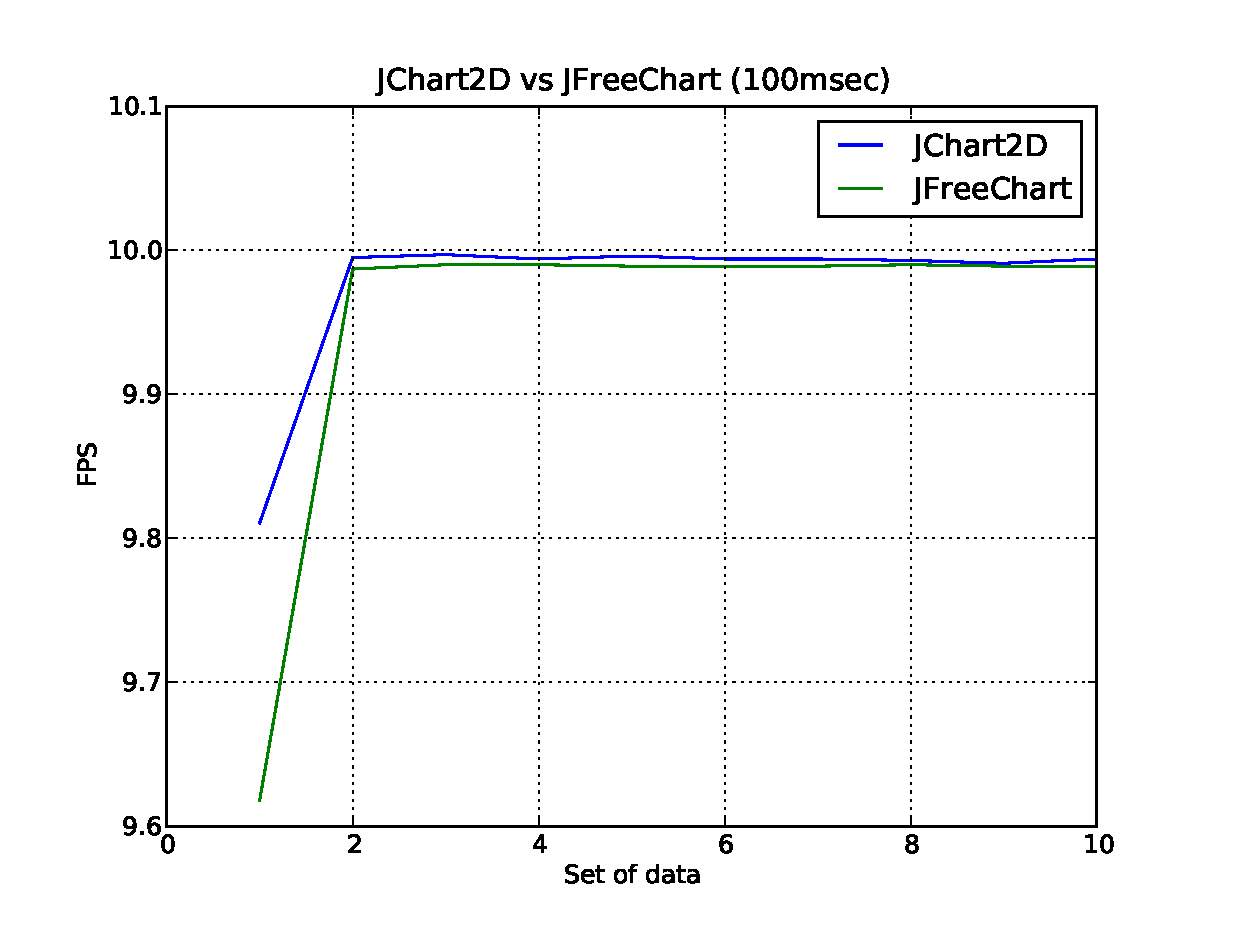
\includegraphics[width=0.32\linewidth, height=!]{../img/java-100}
    \label{fig:java100}
  }
  \subfigure[{10\,[ms] period}]
  {
    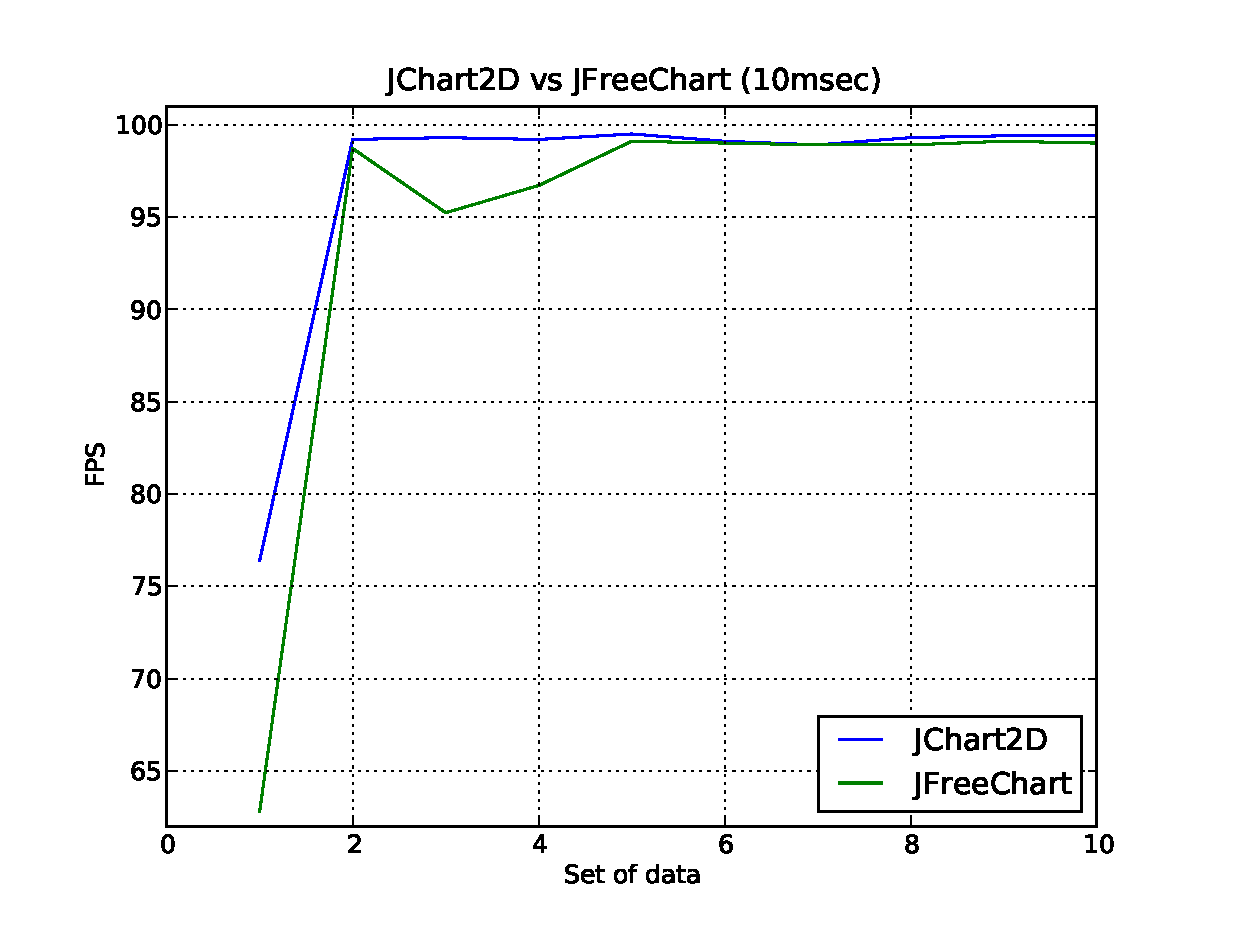
\includegraphics[width=0.32\linewidth, height=!]{../img/java-10}
    \label{fig:java10}
  }
  \subfigure[{1\,[ms] period}]
  {
    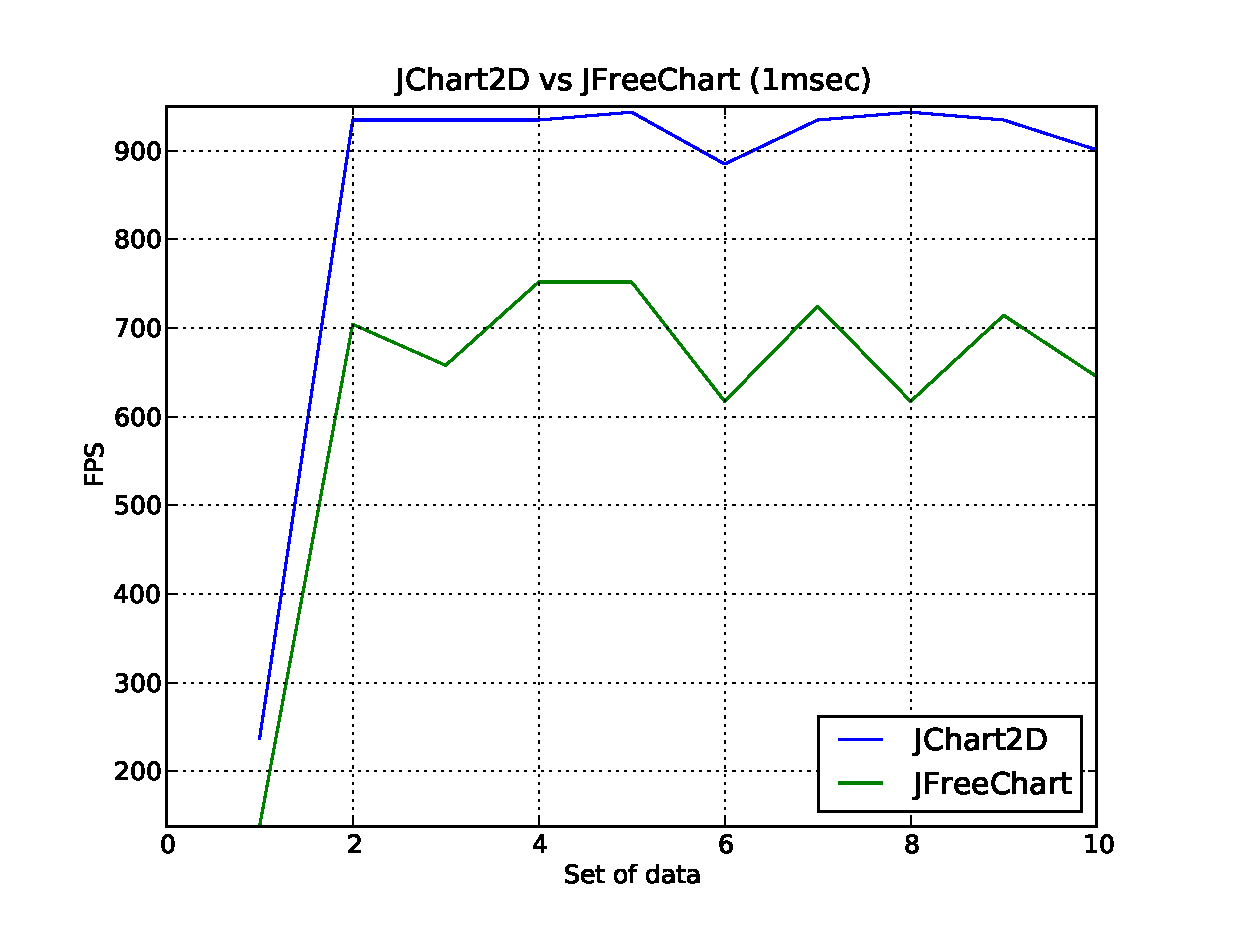
\includegraphics[width=0.32\linewidth, height=!]{../img/java-1}
    \label{fig:java1}
  }
  \label{fig:figure1}
  \caption{JChart2D and JFreeChart comparison plots}
\end{figure}
At first look, JFreeChart shows a inconspicuous lower performance graphing data
with 100\,[ms] of latency time.
There is little difference between the averages
of each library, of the order of $0.024$.
JChart2D has a standard deviation of $0.055$ and a average of $9.975$, which means that
the difference between the FPS are very similar, and has a minimal variation.
JFreeChart has a standard deviation of $0.111$ and a average of $9.952$, which means that
the difference between the FPS at each point has a minimal variation, but is higher compared
to JChart2D.
An important fact is that this latency is slow, so taking it as
reference the scientific data visualization topic we need receiving the data
with a higher frequency.

The second test was performed with an interval of 10\,[ms],
giving the results in figure~\ref{fig:java10}
Decreasing the interval ten times
we see that the difference between the averages of the libraries
increases a little more, we are talking about $2.22$ frames more
for JChart2D.
JChart2D has a standard deviation of $6.861$ and a average of $96.974$, which means that
the difference between the FPS are now higher than in the previous test,
ant it is a large for this same task.
JFreeChart has a standard deviation of $10.717$ and a average of $94.754$, which means that
the difference between the FPS at each point has a noticeable variation, and is higher than the one exhibited by JChart2D.
Also, JChart2D has a regular performance varying a little at each
point, but JFreeChart does not have a regular performance, the three
and four points showed a substantial fall. This fact makes this library unsuitable,
because visualizing scientific data requires a regular
expected behavior.

The third test was performed with a latency time of 1\,[ms].
The resulting FPS of each library are shown in figure~\ref{fig:java1}.
Finally, the difference between FPS for each library
is more noticeable, we are talking about $225.98$ FPS,
and JChart2D outperforms JFreeChart.
JChart2D has a standard deviation of $207.715$ and a average of $858.307$, which means that
the difference between the FPS are now higher related to the two previous tests,
we also note that as the FPS at each point are large values in comparison, so that implies
the big difference between the values.
JFreeChart has a standard deviation of $171.445$ and a average of $632.322$, which means that
this library has a lower standard deviation related to the JChart2D, but the value still being
a large value for a standard deviation; in another hand, the average has a lower value related
the JChart2D average.
Like the previous test, we can look the irregularities of the
JFreeChart performance, at points 3,6, 8 and 10,
so this reaffirms the previous fact that the performance
of JChart2D is most recommendable.

\subsection{Python}

We also compared two Python libraries,
\emph{PyQwt} and \emph{Matplotlib}.
First, the programs start with an interval of data actualization of 100\,[ms],
and the resulting FPS of each library are shown in figure~\ref{fig:python100}.
In this test, as we know in the case of Java, is a kind of non realistic test,
because the data was actualized slowly.
PyQwt has a more stable performance, showing a standard deviation of $0.0004$ that is very close to zero,
keeping the FPS near to 10, but the average of $9.999$ is lower in relation to Matplotlib.
In the side of Matplotlib, the performance has higher and lower points,
but at point number 4 it stabilizes, having an average close to $10.029$.
At first look, Matplotlib is a better choice because it has a better average, but a higher standard variation, $0.010$;
but if the programmer is looking for a library with stable performance,
choosing Matplotlib means taking some risks.

Second, the programs start with an interval of data actualization of 10\,[ms],
and the resulting FPS of each library are shown in figure~\ref{fig:python10}
\begin{figure}%[ht]
  \subfigure[{100\,[ms] period}]{
    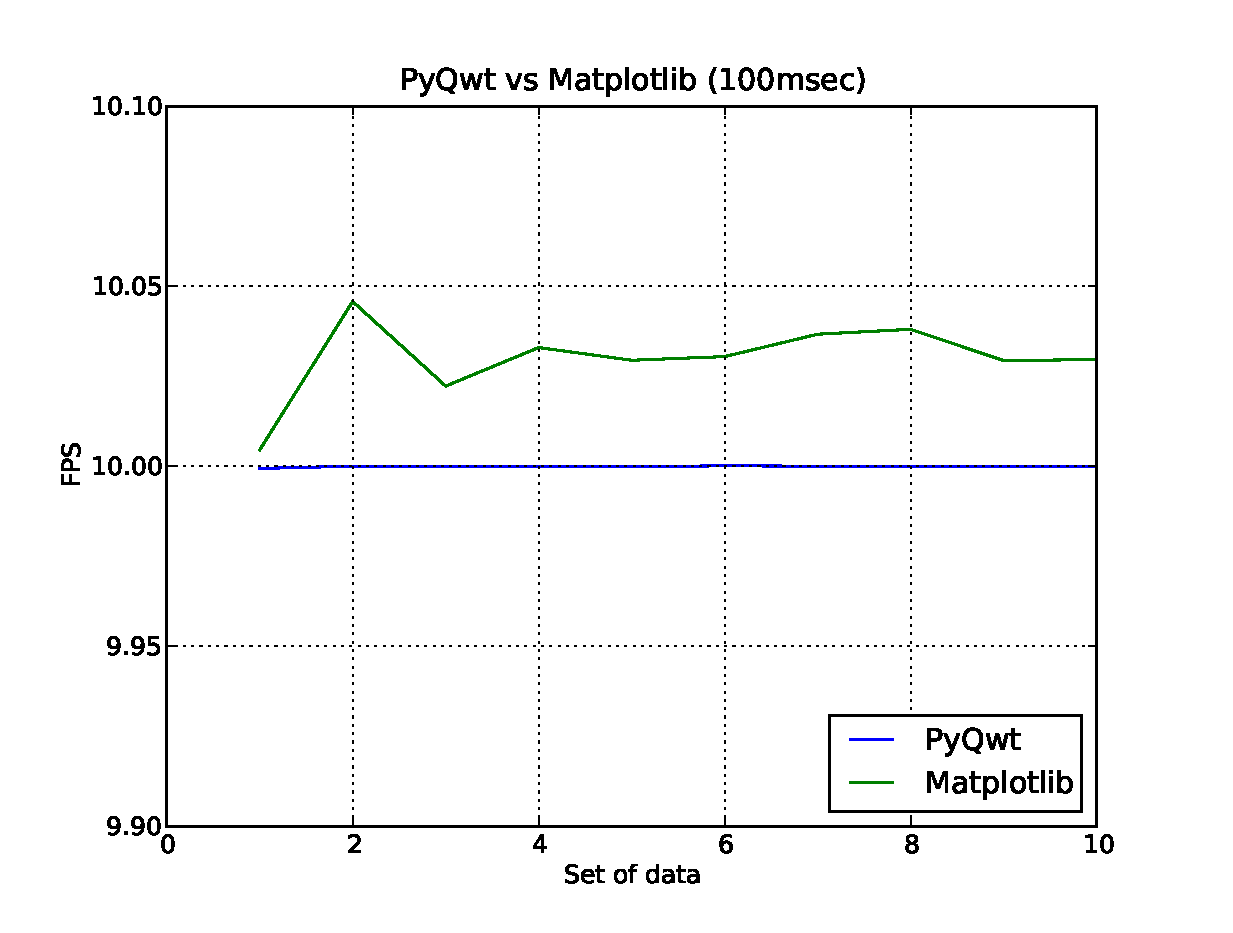
\includegraphics[width=0.32\linewidth, height=!]{../img/python-100}
    \label{fig:python100}
  }
  \subfigure[{10\,[ms] period}]{
    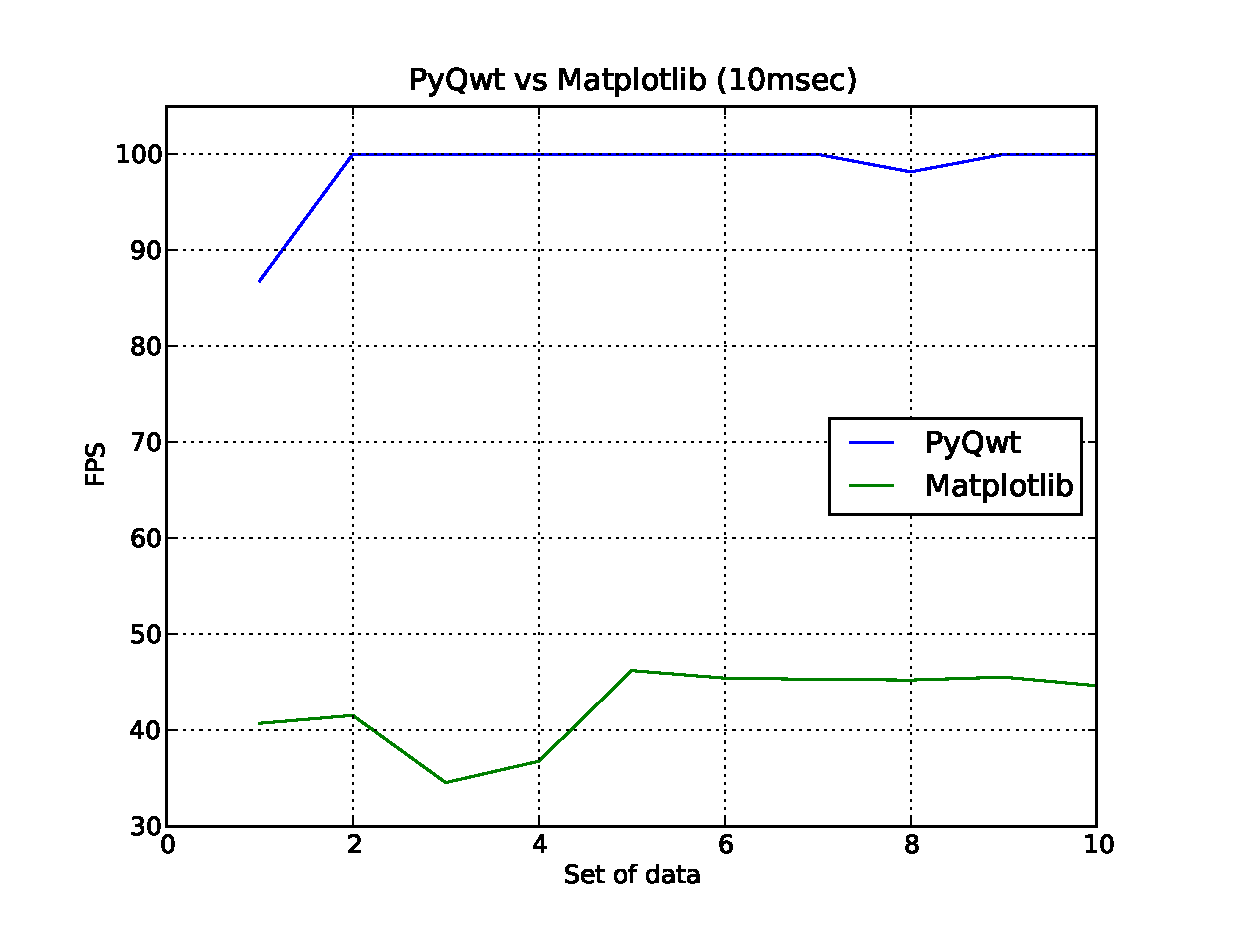
\includegraphics[width=0.32\linewidth, height=!]{../img/python-10}
    \label{fig:python10}
  }
  \subfigure[{1\,[ms] period}]{
    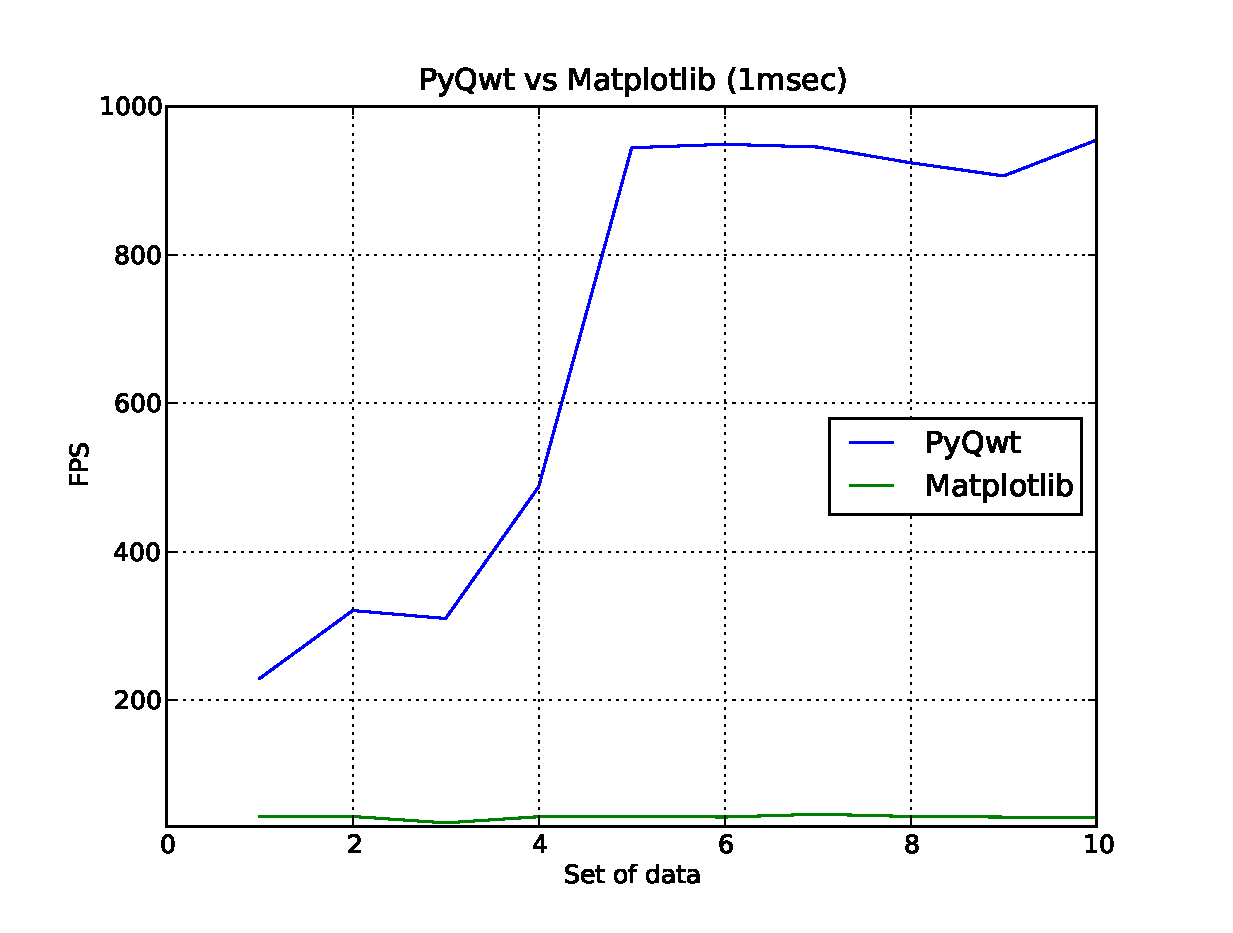
\includegraphics[width=0.32\linewidth, height=!]{../img/python-1}
    \label{fig:python1}
  }
  \label{fig:figure3}
  \caption{PyQwt and Matplotlib comparison plots}
\end{figure}
In this test, a notorious difference comes out,
because the difference between the averages is around $55.90$
FPS, so PyQwt library is the best choice with a average of $98.500$.
Anyway, Matplotlib tries to gain performance from point 5 on forward, but still having
a lower average of $42.598$.
The standard variation of these libraries are very  similar, being $3.932$ and $3.887$ relatively.
On the other hand, the PyQwt has a more constant performance,
which tell us the stability of the library.

Third, the programs start with an interval of data actualization of 1\,[ms],
and the resulting FPS of each library are as given in figure~\ref{fig:python1}.
In this stressed situation the notorious
difference between the performance of PyQwt and Matplotlib
is finally visible,
showing averages of $697.050$ and $42.463$, respectively.
Aside of the performance average, the standard deviation of Matplotlib of $2.809$ is
much lower compared to the PyQwt standard deviation of $300.325$, but this has
direct relation with the obtained values at each point.
As final words it is necessary to say that Matplotlib is not
designed purely to create dynamic plots, its main goal
is to create a lot of graph types in a easy way~\cite{matplotlib-paper}.
On the other hand, PyQwt has the direct binding from the Qwt library
that was designed to obtain high performance in data trending.

\subsection{C++}

Finally, on the C++ side we present the  results of the comparison between
\emph{Qwt} and \emph{wxMathPlot}.
The thread handling in C++ is more efficient,
as it isn't hindered by portability layers.
As a result,
the FPS values obtained are much larger than the ones in previous tests.
FPS in this case are almost equivalent to the data generation rate.

First, the programs start with an interval of data actualization of 100\,[ms] (latency time),
and the resulting \emph{Frames Per Second (FPS)} of each library are shown in figure~\ref{fig:c++100}
\begin{figure}%[ht]
  \subfigure[{100\,[ms] period}]{
    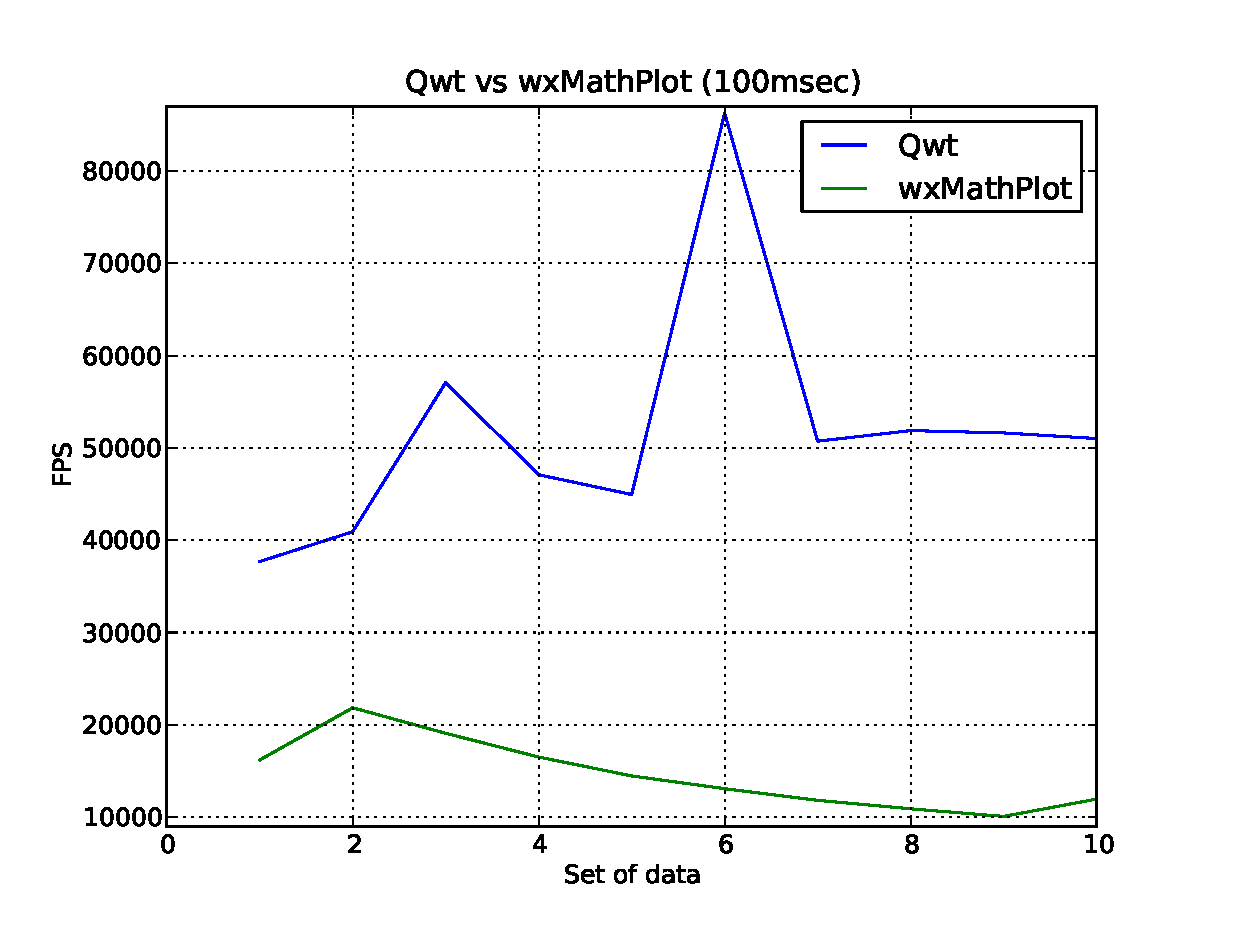
\includegraphics[width=0.32\linewidth, height=!]{../img/c++-100}
    \label{fig:c++100}
  }
  \subfigure[{10\,[ms] period}]{
    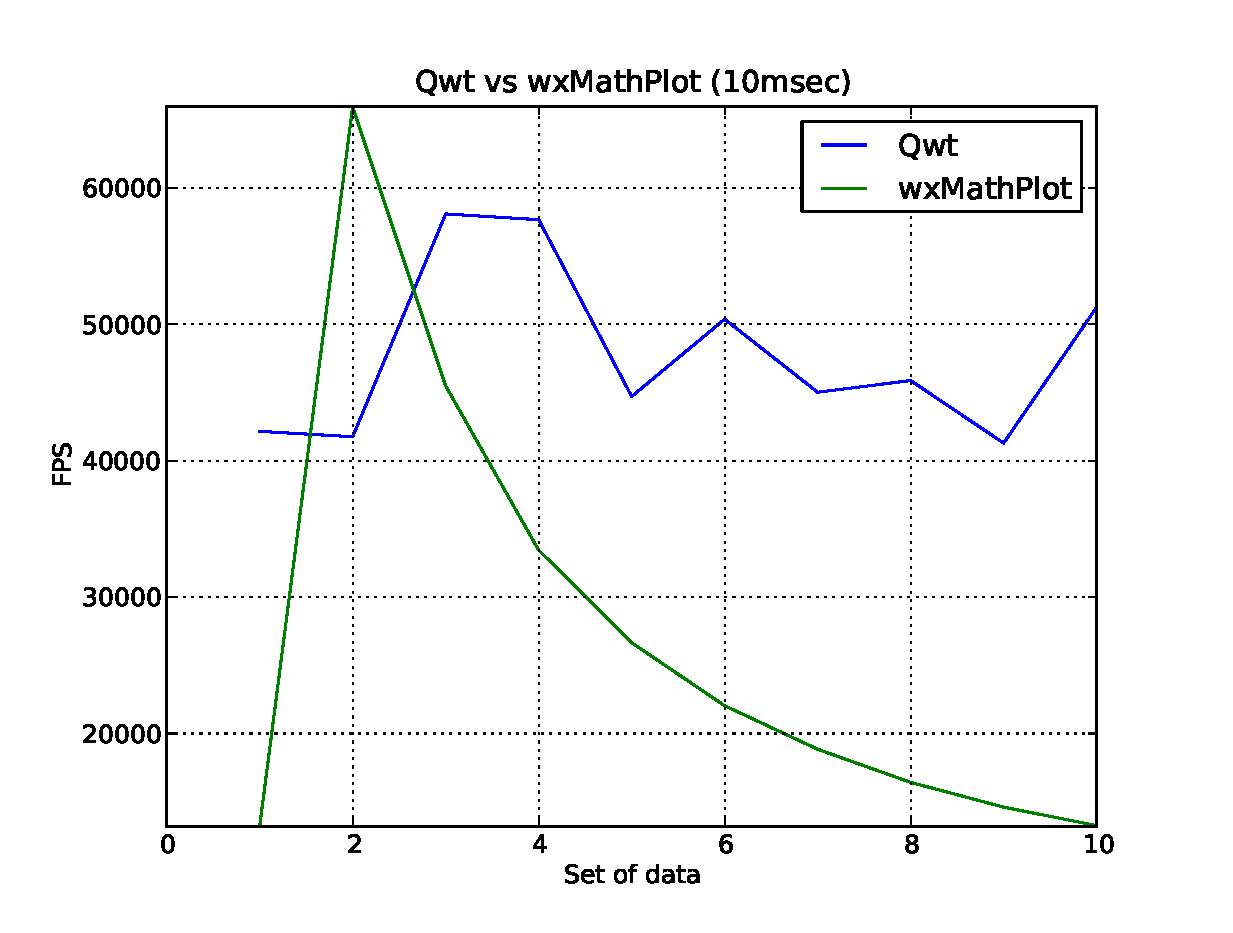
\includegraphics[width=0.32\linewidth, height=!]{../img/c++-10}
    \label{fig:c++10}
  }
  \subfigure[{1\,[ms] period}]{
    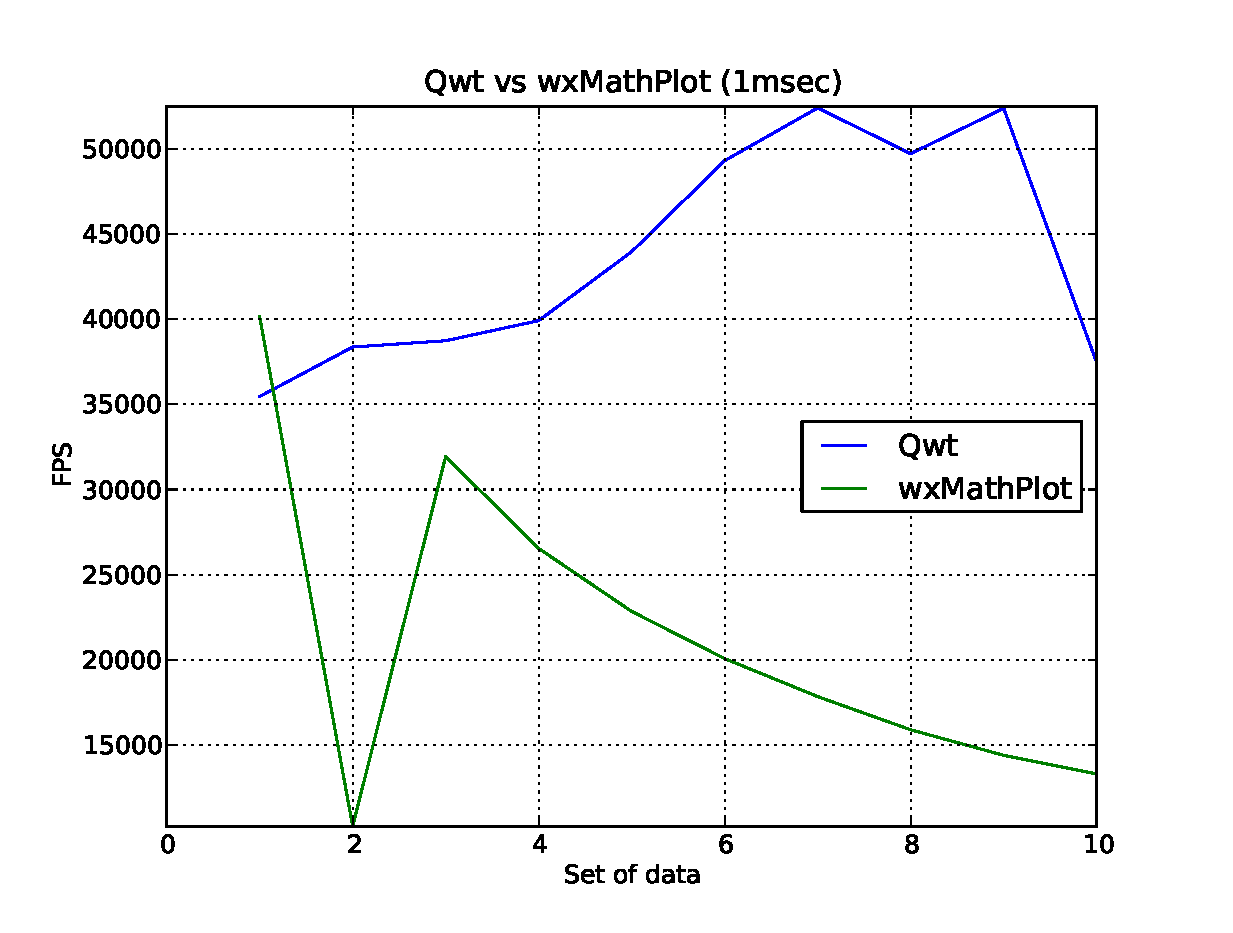
\includegraphics[width=0.32\linewidth, height=!]{../img/c++-1}
    \label{fig:c++1}
  }
  \label{fig:figure4}
  \caption{Qwt and wxMathPlot comparison plots}
\end{figure}
The Qwt library shows better performance than wxMathPlot,
which is reflected in the average of each, $51916.5$ and $14589.5$,
respectively.
On the other hand, the standard deviation tells us about the stability
of each library, in this case wxMathPlot has a decreasing stability,
with a standard deviation of $3605.235$, which is acceptable because
the quantity of data is large enough. Also the Qwt library,
has a more unstable behavior with higher and lower points,
which is defined by their standard deviation of $51916.5$ that is
greater that the previous by one order of magnitude.

Continuing with the test, now with a latency rate of 10\,[ms],
the results in FPS are in figure~\ref{fig:c++10}.
In this case the Qwt performance increases a little, but at
point 2 for example, it is surpassed by wxMathPlot. But in general,
Qwt has better performance with a average of $47830.2$ in
comparison to the $26988.1$ of wxMathPlot.
Respect to the standard deviation wxMathPlot remains the
decreasing stability showing a value of $16242.412$,
that is very high in relation with the standard deviation of
Qwt, $5949.169$. Also Qwt still shows an irregularity
in its performance, due to thread behavior.

Finally we have the last test, that consist in stressing out C++ data trending, with a latency time of 1\,[ms].
The results are in the figure~\ref{fig:c++1}.
In this test, both libraries show very strange behavior, due to the
data Thread actualization with a very low value as is 1\,[ms].
Qwt still wins the match with wxMathPlot, but the irregularity is still present,
because the standard deviation raises to $6271.181$, but in the case of wxMathPlot
that value decreases to $8805.198$, which means that in stability wxMathPlot has the
first place, but related to performance, Qwt wins with a average of $43771.6$
over the wxMathPlot average of $21316.9$.


\subsection{General comments}

The reasons of the lower performance of Python and Java wit respect to C++
are very simple to explain. The execution of every Java program depends on the
Java Virtual Machine.
With respect to Python, PyQwt has simple bindings to the Qwt/C++ library, so they
have a longer path to walk to interact with the final plot.

Another important issue is the threads implementation of each language.
The C++ Standard Library has less features (functionality) and a limited scope
related to the Java Standard Library, but includes native threads libraries.
On the other hand, Python provides low-level primitives for working with multiple threads,
but in difference to C++, Python has POSIX threads and non-POSIX threads.

Software developed in Python is generally slower than Java,
but development time is less with Python,
since Python has dynamic typing and offers built-in high-level data types.
Comparing Java with C++ brings us to similar conclusions.

%%%%%%%%%%%%%%%%%%%%%%%%%%%%%%%%%%%%%%%%%%%%%%%%%%%%%%%%%%%%%
\section{Real Benchmark}
\label{sec:benchmark}
This section presents the result of testing the Sampling System GUI
in a real case scenario at the ALMA Observatory.
The Sampling System GUI is used in the same deployment as
the operations software (ALMASW).
Figure~\ref{fg:deployment} roughly shows the distributed
environment where ALMASW and the Sampling System GUI are deployed.

\begin{figure}%[b]
  \begin{center}
  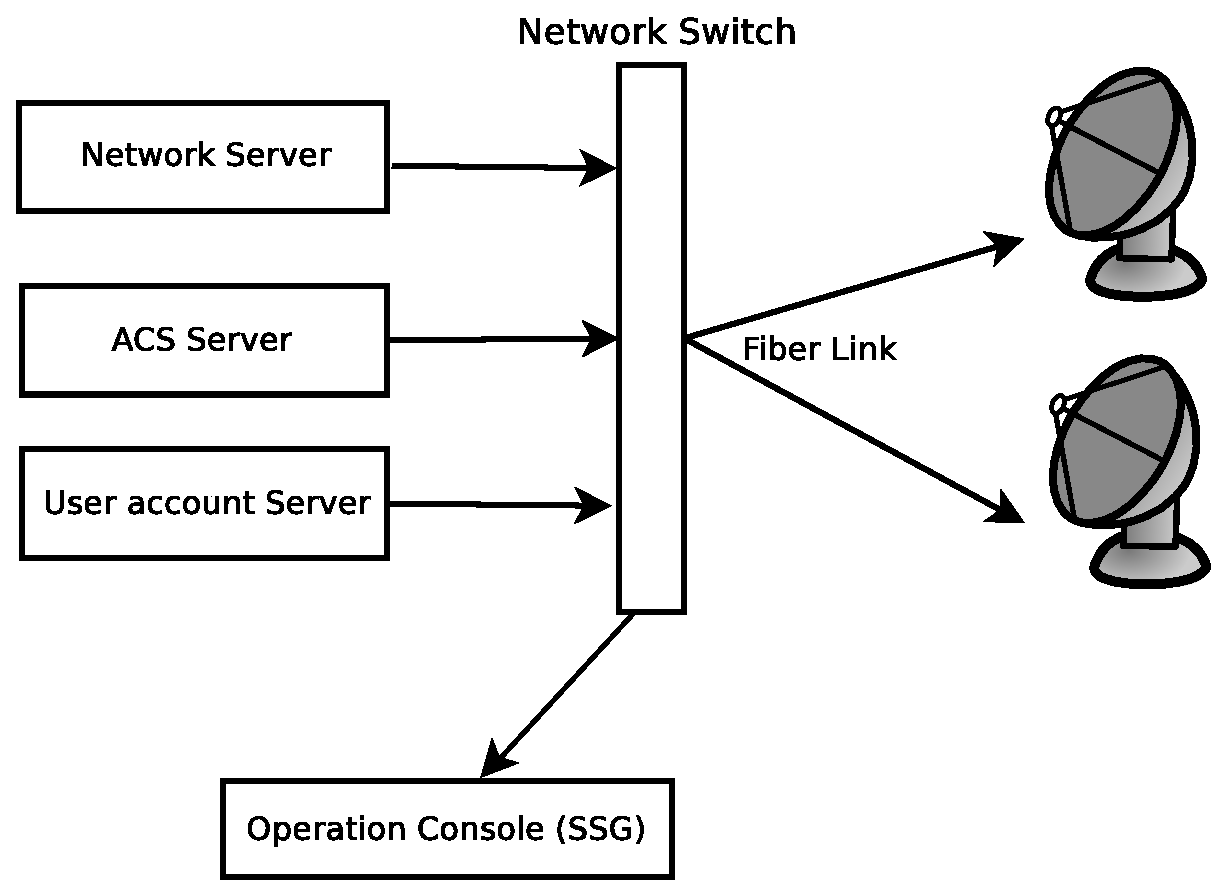
\includegraphics[width=0.50\textwidth]{../img/deployment}
  \end{center}
  \caption{Distributed Deployment}
  \label{fg:deployment}
\end{figure}

ACS and the sampling system run on the ACS server
(figure~\ref{fg:deployment}).
The sampling system GUI is run from the operations console.
This setup was selected to monitor the behavior
of the FrontEnd receiver during its locking routine.
The monitoring setup considered two charts, each with:
\begin{itemize}
\item Five properties being sampled.
\item Sampling frequency of 20\,[Hz].
\item Store a window of 15 minutes of plots.
\item Storing all of the data to disk.
\end{itemize}
20\,[Hz] is the maximum monitoring frequency available in ALMA
since it is limited by its 48\,[ms] period.

The test that was run on the FrontEnd receiver consisted
in locking the band in 0.5\,[GHz] steps over the range of
the four available bands. The test took approximately 4 hours,
time during which the sampling system GUI was
continuously plotting and saving data to disk.
At the time of the test only two antennas were available,
this test should be run again when there are six available antennas
for such purpose. This would demonstrate how the
overall system behaves when increasing the number of distributed
nodes.

The overall result of the Sampling System is positive,
since it met all the engineering requirements for
monitoring during the specified test.
It could cope with the amount of properties and the sampling rates
specified by the engineering division.
Data was properly stored to disk, and the plots
provided a quick look for the data before it was
more thoroughly analyzed.








% real benchmark suite, SSG.


% test cases in a distributed system

%%% Local Variables:
%%% mode: latex
%%% TeX-master: "../article"
%%% End:

%%%%%%%%%%%%%%%%%%%%%%%%%%%%%%%%%%%%%%%%%%%%%%%%%%%%%%%%%%%%%
\section{Conclusions}
\label{sec:conclusions}
% General Conclusions

Better ways of measuring performance,
like the number of data streams that can be displayed at a given FPS
or the impact of smoothly evolving data or scattered points,
should be considered.

Looking backwards, the evolution of the different libraries give the
programmers a lot of ``path to follow'' when starting a new project. The performance
of the actual data trending libraries in different languages is very important
because all of them try to offer ``simple programming'' in this application area.
Comparing the features of the libraries is not so important, because most of them
are rather robust, and those with more features just allow creating more elaborate plots.
Without going further, there are other characteristics to consider, like
``perdurability,'' ``modularity,'' and ``scalability'' of software.
For a long-lived project like ALMA
(and its supporting software ACS)
these characteristics are crucial.
How to estimate the stability and longer range development and maintenance
of open source software on which something like ACS is based
is still very much an open question.

In section~\ref{sec:gbenchmark} we saw benchmarks of a couple of graphic libraries
in the three languages that ACS uses, C++, Java, and Python.
The benchmark shows the behavior of these libraries in three levels
of stressed environments, giving us data to discriminate among them.
Anyway, this is not a final decision, because one benchmark is not enough to test the real
performance of a graphical library, but it is a good start to help discriminating them with the previous
basic functionality (plotting random data).
Also,
other important characteristics haven't been considered in detail.
For a long-lived protect like ALMA
(and its supporting ACS package)
using stable, well-maintained base software is crucial.

Finally, in section~\ref{sec:benchmark} we can see the performance of
the existing scientific data visualization tool, developed by the Computer Systems Research Group (CSRG),
and giving us the chance to analyze a real application in a real distributed system such as the
ALMA project.

%%% Local Variables:
%%% mode: latex
%%% TeX-master: "../article"
%%% End:


%%%%%%%%%%%%%%%%%%%%%%%%%%%%%%%%%%%%%%%%%%%%%%%%%%%%
\appendix    %>>>> this command starts appendixes
%%%%%%%%%%%%%%%%%%%%%%%%%%%%%%%%%%%%%%%%%%%%%%%%%%%%

%%%%%%%%%%%%%%%%%%%%%%%%%%%%%%%%%%%%%%%%%%%%%%%%%%%%%%%%%%%%%
\acknowledgments     %>>>> equivalent to \section*{ACKNOWLEDGMENTS}

This work and the associated research has been conducted with funds granted by CONICYT, specifically ALMA-CONICYT grant \#31090034 and \#31080031.
Horst H. von Brand's work was also supported in part
by Centro Cient\'\i fico-Tecnol\'ogico de Valpara\'\i so (CCTVal) grant FB0821.
Without their help, this work would have been impossible.

%%%%%%%%%%%%%%%%%%%%%%%%%%%%%%%%%%%%%%%%%%%%%%%%%%%%%%%%%%%%%
%%%%% References %%%%%
\hfill
\bibliography{report}   %>>>> bibliography data in report.bib
\bibliographystyle{styles/spiebib}   %>>>> makes bibtex use spiebib.bst

\end{document}

%%% Local Variables:
%%% mode: latex
%%% TeX-master: t
%%% End:
